% THIS TEMPLATE IS A WORK IN PROGRESS
% Adapted from an original template by faculty at Reykjavik University, Iceland

\documentclass{scrartcl}
\input{File_Setup.tex}
\usepackage{graphicx,epsfig,array, booktabs, pdflscape}
\usepackage{float, longtable}
\usepackage[utf8]{inputenc}
\usepackage[table]{xcolor}
\hypersetup{
   colorlinks   = true,                               %Colours links instead of ugly boxes
   urlcolor     = blue,                               %Colour for external hyper links
   linkcolor    = blue,                               %Colour of internal links
   citecolor    = red,                                %Colour of citations
   setpagesize  = false,
   linktocpage  = true,
}
\graphicspath{ {fig/} }



\renewenvironment{abstract}{
    \centering
    \textbf{Abstract}
    \vspace{0.5cm}
    \par\itshape
    \begin{minipage}{0.7\linewidth}}{\end{minipage}
    \noindent\ignorespaces
}
% ------------------------------------------------------------------------------------------------------------------------

\begin{document}
\begin{titlepage}
	\centering
	
\includegraphics[width=0.6\textwidth]{GW_logo.eps}\par
	\vspace{2cm}
	%%%% COMMENT OUT irrelevant lines below: Data Science OR Computer Science OR none
	{\scshape\LARGE Data Science Program \par}
	\vspace{1cm}
	{\scshape\Large Capstone Report - Fall 2025\par}
	%{\large \today\par}
	\vspace{1.5cm}
	%%%% PROJECT TITLE
	{\huge\bfseries Smart School Food Service Analysis: AI-Driven Demand Forecasting and Waste Reduction Using Fairfax County Public Schools Data\par}
	\vspace{2cm}
	%%%% AUTHOR(S)
	{\Large\itshape Jupiter Kang,\\ Crystal Kao,\\ Alonso Romero\\}\par
	\vspace{1.5cm}
	supervised by\par
	%%%% SUPERVISOR(S)
	Amir Jafari

	\vfill

    \newpage

	\begin{abstract}
	    Food waste in U.S. public schools presents a significant economic and environmental challenge, with approximately 530,000 tons of food discarded annually, resulting in \$1.2 billion in losses. Fairfax County Public Schools (FCPS) in Virginia seeks to address this issue by leveraging data-driven insights to optimize their food service operations. Despite widespread availability of digital data from Point-of-Sale (POS) systems and kitchen production records, most districts—including FCPS—lack the analytical tools necessary to effectively utilize this information. This project analyzes FCPS data from March to May 2025 to uncover patterns in food consumption, identify inefficiencies, and recommend actionable strategies for reducing waste. Key research objectives include evaluating a la carte item popularity at the school level, assessing participation trends through year-over-year comparisons, and segmenting data by FCPS regions and school level. Through advanced data analytics, this study aims to support FCPS in making informed, efficient, and sustainable decisions for school meal planning and delivery.
	\end{abstract}
	\vfill
% Bottom of the page
\end{titlepage}
\tableofcontents
\newpage
% ------------------------------------------------------------------------------------------------------------------------
\section{Introduction}

 Food waste in institutional food service is a critical economic and environmental challenge. In large public systems like Fairfax County Public Schools (FCPS), the complexity of predicting daily student demand often leads to substantial overproduction and resource misallocation. Traditional manual planning methods lack the precision to account for variables such as menu popularity and enrollment shifts, resulting in a system where waste is frequently treated as an unavoidable cost of operations.

This study addresses this gap by developing an intelligent analytics and optimization framework specifically for school food systems. By combining Point-of-Sale (POS) data with production records, we moved beyond simple forecasting to create a prescriptive Mixed-Integer Linear Programming (MILP) model.

Building upon the initial objectives of creating a data-driven decision support system, this research achieved the following specific contributions:

\begin{itemize}

    \item \textbf{Optimization of Production Quantities}: We developed a mathematical model to minimize waste and cost, ensuring food availability aligns with actual demand rather than static averages.

    \item \textbf{Nutritional Constraint Integration}: The model incorporates dietary parameters to ensure that waste reduction strategies do not compromise the nutritional standards mandated for student meals.

    \item \textbf{Cost-Effectiveness Analysis}: We quantified the economic impact of optimization, providing a system-wide feasibility analysis that identifies potential savings of over \$1.8 million.

    \item \textbf{Operational Scalability}: We evaluated the model across different school sizes (500–3,500+ students) to provide tailored recommendations for diverse operational environments.
\end{itemize}

By validating this framework against real-world FCPS data, this work offers a scalable solution for reducing pre-consumer waste and optimizing budget allocation in the public sector.

% ------------------------------------------------------------------------------------------------------------------------
\section{Problem Statement}

Food Waste in U.S. public schools has been a major issue, and FCPS in Virginia wants to find ways to reduce food waste for their county. The main goal of our analysis is to provide the following: 

\

A recommendation list of foods in order to optimize the spending by creating a customized budget that is more efficient and data driven, with breakdowns by region, school level, and individual schools.


% ------------------------------------------------------------------------------------------------------------------------

\section{Related Work}

\textbf{Behavioral Diagnostics and Operational Interventions}
Current research on school food waste predominantly focuses on behavioral diagnostics and manual quantification. Studies by Martins et al. \cite{factors} and Rada et al. \cite{rada} identify the cafeteria environment as a primary driver of waste, though they attribute this to different factors. While Martins et al. emphasize the role of supervision, finding that the physical presence of teachers reduced waste rates \cite{factors}. Rada et al. focus on the demographic capabilities of the students, noting a shift from organic waste in primary schools to packaging waste in high schools \cite{rada}. Complementing these diagnostic studies, Elnakib et al. \cite{elnakib} demonstrated that operational interventions, such as staff training and the "Smarter Lunchrooms" movement, could yield a 7\% reduction in waste.

However, a common limitation across these studies is their reliance on reactive measures. Martins et al. and Rada et al. rely on ex-post manual auditing, which diagnoses the problem but does not predict it \cite{factors, rada}. Similarly, the interventions proposed by Elnakib et al. rely heavily on human consistency and staff adherence \cite{elnakib}. The present study diverges from these approaches by proposing a predictive, automated framework. Rather than relying on behavioral nudges or manual audits, our work utilizes optimization to prevent surplus production at the source, independent of daily staff variance.

\textbf{Optimization in Food Supply Chains}
While Mixed-Integer Linear Programming (MILP) is a well-established tool in food supply chains, its application has historically been bifurcated between upstream agriculture and downstream waste logistics, bypassing the specific niche of cafeteria production planning.

On the downstream side, existing literature utilizes MILP primarily for post-consumer waste management. For instance, Kabadurmus et al. applied a bi-objective MILP to optimize the flow of waste to reuse centers \cite{kabadurmus}, while Korcyl, Ksi{\k{a}}{\.z}ek, and Gdowska utilized it for vehicle routing in waste collection \cite{korcyl}. Both studies confirm MILP’s efficacy in handling heterogeneous constraints and minimizing network costs. However, they address waste only after it has been generated. Our study adapts these mathematical formulations but shifts the temporal focus to the pre-consumer stage, using MILP to optimize procurement and prevent waste generation before it occurs.

On the upstream side, optimization has been applied to agricultural harvest scheduling. G{\"u}nder et al. research comparing Evolutionary Algorithms (EA) against standard MILP found that while EA handles biological non-linearity better, MILP remains the superior tool for cost-based, resource-constrained environments \cite{gunder}. This validates our selection of MILP for the school cafeteria setting, which functions more like a discrete manufacturing line than a biological system. Furthermore, Akkerman et al. demonstrated the utility of MILP in balancing the "triple bottom line" (cost, environment, quality) in institutional catering distribution \cite{akkerman}. Our work builds upon this multi-objective foundation but specifically tailors the constraints to the unique budget cycles and nutritional requirements of a public school system, creating a model that is both mathematically robust and operationally feasible for school administrators.

% ------------------------------------------------------------------------------------------------------------------------

\section{Solution and Methodology}

For our project, we used Mixed-Integer Linear Programming (MILP) to provide us with optimized values for recommended menu item count to be ordered. Integer linear programming “\textit{involves the optimization of linear equations by assigning integer values to each variable, thus allowing for optimal solutions that are integral rather than fractional}” \footnote{\href{https://www.complexica.com/narrow-ai-glossary/integer-programming}{Integer Linear Programming}}. For this instance, using integers for values produced is ideal as menu items should not be served as fractions, but rather the whole amount. “\textif{The goal of this technique is to maximize profit while minimizing cost and resources}” \footnote{\href{https://www.complexica.com/narrow-ai-glossary/integer-programming}{Integer Linear Programming}}.

\subsection{Mixed-Integer Linear Programming}

Our MILP model to help FCPS cafeteria managers reduce food waste by selecting the optimal number of menu items while staying within budget. It is also important to consider uncertainty. Sensitivity allows for different variations of the model, which can help address parameter uncertainty \cite{algo_milp}. We implemented specific budget scenarios (80\%, 100\%, and 120\% of the baseline budget) in our model, which provides a complete map of possible solutions as parameters change. Following the sensitivity analysis framework from \cite{ren}, we tested the robustness of our model by varying key parameters. Specifically, we analyzed how the optimal production quantities changed in response to fluctuations in student demand. Since a parameter such as student demand often fluctuates, running different scenarios is ideal to maintain a safe production plan \cite{mathmodel}. The following is from our baseline analysis.

\begin{itemize}
    \item \textit{Decision Variables}: Let $x_j$ be the integer quantity of menu item $j$ to be produced.
    \item \textit{Parameters}: A critical component of the MILP model is the accurate definition of cost parameters. A significant challenge in utilizing raw financial data is that school county budget documents list expenditures as a grand total, no specified expenses that contribute to the grand total. To overcome this lack of granularity and define a usable parameter for the objective function, we derive the effective unit production cost for each item based on historical service data. The unit production cost, denoted as $c_j$ for item $j$ is calculated as the ratio of the total production cost to the total quality served. Utilizing the FCPS dataset provided, this is defined as:

    \begin{equation}
        c_j = \frac{\text{Production Cost Total}_j}{\text{Served Total}_j}
    \end{equation}

    Where:
    \begin{itemize}
        \item $\text{Production Cost Total}_j$: represents the aggregate cost incurred to produce the volume of item $j$ offered.
        \item $\text{Served Total}_j$: represents the total count of item $j$ actually served to students (reimbursable plus non-reimbursable).
    \end{itemize}

    Then for the objective function, the parameters are:
    \begin{itemize}
        \item $c_j$: The unit production cost for item $j$.
        \item $w_j$: The waste penalty associated with item $j$ (derived from historical leftover rates).
        \item $d_j$: The predicted demand for item $j$.
    \end{itemize}

    \item \textit{Objective Function}: The objective is to minimize the total cost, balancing the financial cost of meals and the environmental cost of waste. Applying Afshar et al. concept of 'Value of Lost Load' to a school cafeteria setting, our model assigns a penalty weight to unserved meals that exceeds the cost of food waste \cite{afshar}. This ensures that waste reduction does not come at the expense of student food security. The objective function is:

    \begin{equation}
        \text{Minimize Z} = \sum^n_{i=1}\sum^m_{j=1}(c_{ij} + \lambda w_{ij})x_{ij}
    \end{equation}

    While the waste penalty parameter ($\lambda$) was set to 0.1 to balance environmental and financial goals, this value lacks empirical grounding in actual disposal costs. As the model's optimal outputs fluctuate significantly based on this weight, the reported results are conditional on this specific setting. Future operators should adjust $\lambda$ to strictly align with their district's operational costs and environmental priorities.

    \item \textit{Constraints}: Our model includes production and financial constraints that penalize potential waste to ensure appropriate amounts of food are produced. To align production with student needs and minimize waste, we used a production bounds constraint. This constraint keeps production within a defined range. The range is based on estimated demand:

    \begin{equation}
        L_{s,j} \le x_{s,j} \le U_{s,j}  \ \ \ \ \ \forall s, \forall j
    \end{equation}

    \begin{table}[H]
        \centering
        \begin{tabular}{cc}
            \toprule
            \textbf{Student Population} & \textbf{Production Bounds $(L, U)$} \\
            \midrule
            0--499 & (0.80, 1.20) \\
            500--999 & (0.85, 1.15) \\
            1000--1499 & (0.90, 1.10) \\
            1500--1999 & (0.95, 1.05) \\
            2000--2499 & (0.96, 1.04) \\
            2500--2999 & (0.97, 1.03) \\
            3000--3499 & (0.98, 1.02) \\
            3500+ & (0.99, 1.01) \\
            \bottomrule
        \end{tabular}
        \caption{Production Bounds Based on School Size}
        \label{tab:production_bounds}
    \end{table}

\end{itemize}

In our optimization model, we scale the bounds by size multipliers tied to each school's student population (\autoref{tab:production_bounds}). We see that smaller schools have a longer range than the larger schools. Schools with smaller populations are more volatile, as a small change in daily events can result in a significant impact on the waste percentage. For example, a school of 500 students has a flu outbreak one day, and 50 students call in sick; that is a 10\% reduction in demand that day. A wider buffer accounts for this unpredictability. On the other hand, a school of 3000 students with 50 students calling out on any given day would result in a 1.6\% reduction in demand. The buffer would be tighter as attendance is more stable. This is represented by:

\begin{equation}
    \begin{aligned}
        L_{s,j} &= \alpha_s \cdot d_{s,j} \\
        U_{s,j} &= \beta_s \cdot d_{s,j}
    \end{aligned}
\end{equation}

Here, $d_{s,j}$ represents the demand for item $j$ at school $s$. In addition to these production bounds, we require that the production quantities, represented by the decision variables, be non-negative integers, enforced by:

\begin{equation}
    x_{s,j} \in \mathbb{Z}^+ \quad \forall s, \forall j
\end{equation}

Finally, we included two budget constraints in the model: a per-school budget constraint ($B_s$), and a system-wide total budget constraint ($B_{total}$):

\begin{equation}
    \sum_{j} (c_{j} \cdot  x_{s,j}) \leq B_{s}
    \label{eq:school_budget}
\end{equation}

\begin{itemize}
    \item $c_j$: The unit production cost for item $j$.
    \item $x_{s,j}$: Quantity of items produced by school $s$.
    \item $B_s$: The maximum budget allocated to school $s$.
\end{itemize}

The per-school budget constraint ensures equity across all the schools in the system. It prevents larger schools from "hoarding" the budget, ensuring every school has enough funds to meet its specific needs.

\begin{equation}
    \sum_{s}\sum_{j} (c_{j} \cdot x_{s,j}) \leq B_{total}
    \label{eq:total_budget}
\end{equation}

The system-wide budget constraint ensures sustainability. It ensures that the spending across the county does not exceed the allocated \$139,144,760 budget \cite{fcpsbudget}. Implementing a system-wide budget constraint is ideal, as the entire school system must remain within the total budget while optimizing individual schools. This allows the model to optimize the allocation of funds between purchasing higher-quality (less wasteful) ingredients and the labor needed to prepare them, ensuring that the solution remains financially feasible \cite{cobuloglu}.

\begin{table}[H]
    \centering
    \renewcommand{\arraystretch}{1.5}

    \begin{tabular}{|l|l|l|r|}
    \hline
        \rowcolor{lightgray!50} % Darker gray for the header row
        \textbf{School} & \textbf{meal\_type} & \textbf{food\_item} & \textbf{recommended\_quantity} \\ 
        \hline
        aldrin elementary & Breakfast & Apple Juice(Each) & 1158 \\
        \hline
        aldrin elementary & Breakfast & Orange Tangerine Juice(Each) & 626 \\
        \hline
        aldrin elementary & Breakfast & Mini Maple Pancakes(Packages) & 534 \\
        \hline
        aldrin elementary & Breakfast & 1\% White Milk(Each) & 522 \\
        \hline
    \end{tabular}
    \caption{Results of the Mixed Integer Linear Program}
    \label{tab:rectable}
\end{table}

\autoref{tab:rectable} shows the results as a csv file generated by the model. It lists each school, for each meal type and the individual menu item and its recommended quantity. This provides the user with an optimal amount of each item in order to reduce waste while saving money.

\subsection{Regression Analysis}

To further investigate the factor of the school food service system, we conducted a regression analysis to predict the production cost. This analysis serves as an additional tool to validate cost behaviors descriptively.

\subsubsection{Ordinary Least Squares}

We utilized the Ordinary Least Squares (OLS) regression to estimate the relationship between a dependent variable(Y) and one or more independent variables (X) by minimizing the sum of the squared differences (residuals) between the observed values and the values predicted by the linear model \cite{Wooditch2021}.

The general linear model is defined as \cite{james2021ISL}:
\begin{equation}
    Y_i = \beta_0 + \sum^k_{j=1}\beta_jX_{ij}+\epsilon_i
\end{equation}

Where:
\begin{itemize}
    \item $Y_i$ represents the dependent variable (e.g., Production Cost) for school $i$.
    \item $\beta_0$ is the intercept, representing fixed operational baselines.
    \item $\beta_j$ represents the marginal impact of the $j$-th independent variable.
    \item $X_{ij}$ represents the independent variables (e.g., student enrollment, waste metrics).
    \item $\epsilon_i$ is the error term, assumed to be normally distributed $\epsilon \sim N(0, \sigma^2)$.
\end{itemize}

\subsubsection{Objective Function and Implementation}

The primary goal of OLS method is to determine the optimal values for the coefficients $\hat{\beta_0}$ and $\hat{\beta_1}$ that minimize the Sum of Squared Residuals (SSR). A lower SSR value indicates a better-fitting model that makes more accurate predictions. The objective function is mathematically formulated as \cite{jameslr}:

\begin{equation}
    \min_{\beta_0, \beta_1} S(\beta_0, \beta_1) = \sum_{i=1}^{n} (y_i - \hat{y}_i)^2 = \sum_{i=1}^{n} (y_i - (\beta_0 + \beta_1 x_i))^2
    \label{eq:ols_obj}
\end{equation}


To validate the model’s accuracy and reliability on predicting production cost, the methodology strictly incorporates a cross-validation protocol. The dataset is split into a training set (80\%) and a test set (20\%).The algorithm exclusively utilized the training set to derive the coefficients. Then these learned patterns are applied to the test set to generate the prediction model. Finally, the predictions are compared with the original production cost in the test set to quantify how accurate and how reliable the model is. By minimizing this function, we ensure that the predicted production costs ($\hat{y}$) are as close as possible to the historical data provided by FCPS.

\subsubsection{Regression Future Pathway}

Although the regression component operates independently of the MILP optimization, it provides essential statistical validation for the cost parameters utilized in the optimization constraints. Currently this regression framework is \textit{descriptive},providing a statistical explanation of historical costs. In our future research, we can use our regression outputs inside the optimization models to explore decisions or predictions under different constraints \cite{Elmachtoub2017}.

The coefficients derived from the OLS analysis ($\beta_j$)serve as the objective function parameters for a Linear Programming (LP)problem. For example, once the marginal cost of waste ($\beta_{waste}$) is empirically determined, an optimization solver can be formulated to minimize total operational cost $Z$:

\begin{equation}
    \text{Minimize } Z = \sum_{i=1}^{n} (\beta_{prod} \cdot x_{i,prod} + \beta_{waste} \cdot x_{i,waste})
\end{equation}


Subject to demand and capacity constraints:
\begin{align}
    x_{i,prod} &\geq D_{i} \quad \forall i \in \text{Schools} \\
    x_{i,prod} &\leq C_{cap}
\end{align}


By feeding the empirically derived regression coefficients into the optimization model, the system evolves from merely identifying inefficiencies to algorithmically prescribing production quotas that minimize waste and maximize budgetary efficiency.

% ------------------------------------------------------------------------------------------------------------------------
\section{Results}

The results section details your metrics and experiments for the assessment of your solution. It then provides experimental validation for your approach with visual aids such as data tables and graphs. In particular, it allows you to compare your idea with other approaches you've tested, for example solutions you've mentioned in your related work section.

\subsection{Experimentation protocol}

\textbf{Actual Annual Cost}: Calculates the realized production costs for the month of May and multiplied by 10 to represent the annual school year. The formula is represented as:
\begin{equation}
    AAC = \sum \text{production costs} * 10
\end{equation}

\textbf{Average Daily Demand}: Calculates the day-by-day average of each individual menu item demand from all the schools in the school system. The formula is represented as:
\begin{equation}
    \text{avg\_bf\_demand} = \frac{\sum \text{served reimbursable}}{\text{\# of days}} \ \ \ \  \ \text{avg\_ln \_demand} = \frac{\sum \text{served reimbursable}}{\text{\# of days}}
\end{equation}

\textbf{Item Popularity}: Calculates how popular an item is within its meal category. The formula is represented as:

\begin{equation}
    \text{bf\_pop\_prop} = \frac{\text{bf popularity}}{\text{bf total served}} \ \ \ \ \ \ \text{ln\_pop\_prop} = \frac{\text{ln popularity}}{\text{ln total served}}
\end{equation}

\textbf{Leftover Rate}: Calculates the leftover rate of individual items. The formula is represented as:

\begin{equation}
    (\frac{\text{Total Leftover}}{\text{Total Offered}}) \times 100
\end{equation}

\textbf{Minimized Cost}: Calculates the optimizer model to find a solution that is both low in cost and less prone to waste. The formula is represented as:

\begin{equation}
    C_T = \text{meal\_cost} + (0.1 \cdot \text{waste penalty}[j])
\end{equation}

\textbf{Monthly Food Cost}: Calculates the cost based on the specific item costs for a month. Where the recommended item quantity is multiplied by the item unit cost. The formula is represented as: 

\begin{equation}
    C_M = R_Q \cdot C_{\text{item}}
\end{equation}

\textbf{Net Consumption}: Calculates the amount that was actually eaten. The formula is represented as:

\begin{equation}
    \text{Net Consumption} = \sum \text{Served Reimbursable} - \sum \text{Discarded Total}
\end{equation}

\textbf{Optimized Annual Cost}: Calculates the total production cost of the menu items by the optimized quantity multiplied by the unit cost altogether multiplied by 10 to represent the annual school year. The formula is represented as:

\begin{equation}
    OAC = \sum(R_Q \cdot c_{\text{item}}) \cdot 10
\end{equation}

\textbf{Percent Savings}: Calculates the percentage of savings against the actual annual cost. The formula is represented as:

\begin{equation}
    \text{Savings \%} = \frac{S}{AAC} \cdot 100
\end{equation}

\textbf{Recommended Item Quantity}: Calculates the general menu item quantity into specific item counts. Where the optimal quantity is multiplied by the menu item proportion. The formula is represented as:

\begin{equation}
    R_Q = \text{optimal quantity} \cdot \text{item proportion}
\end{equation}

\textbf{Total Savings/Loss}: Calculates the total savings or loss from the actual recorded costs from the optimized costs. The formula is represented as:

\begin{equation}
    S = AAC - OAC
\end{equation}

\textbf{Unit Cost}: Calculates the individual production costs of making a menu item for the breakfast and lunch for the schools in the system. The formula is represented as:

\begin{equation}
    c_{\text{item}} = \frac{\text{production cost}}{\text{offered}}
\end{equation}

\textbf{Budget Constraint}
To make our model provide realistic results, we have considered a budgetary constraint. Fairfax County Public Schools allocates a dedicated amount to the Food and Nutrition Services from its overall annual budget \cite{fcpsbudget}.

\begin{figure}[H]
	\begin{center}
		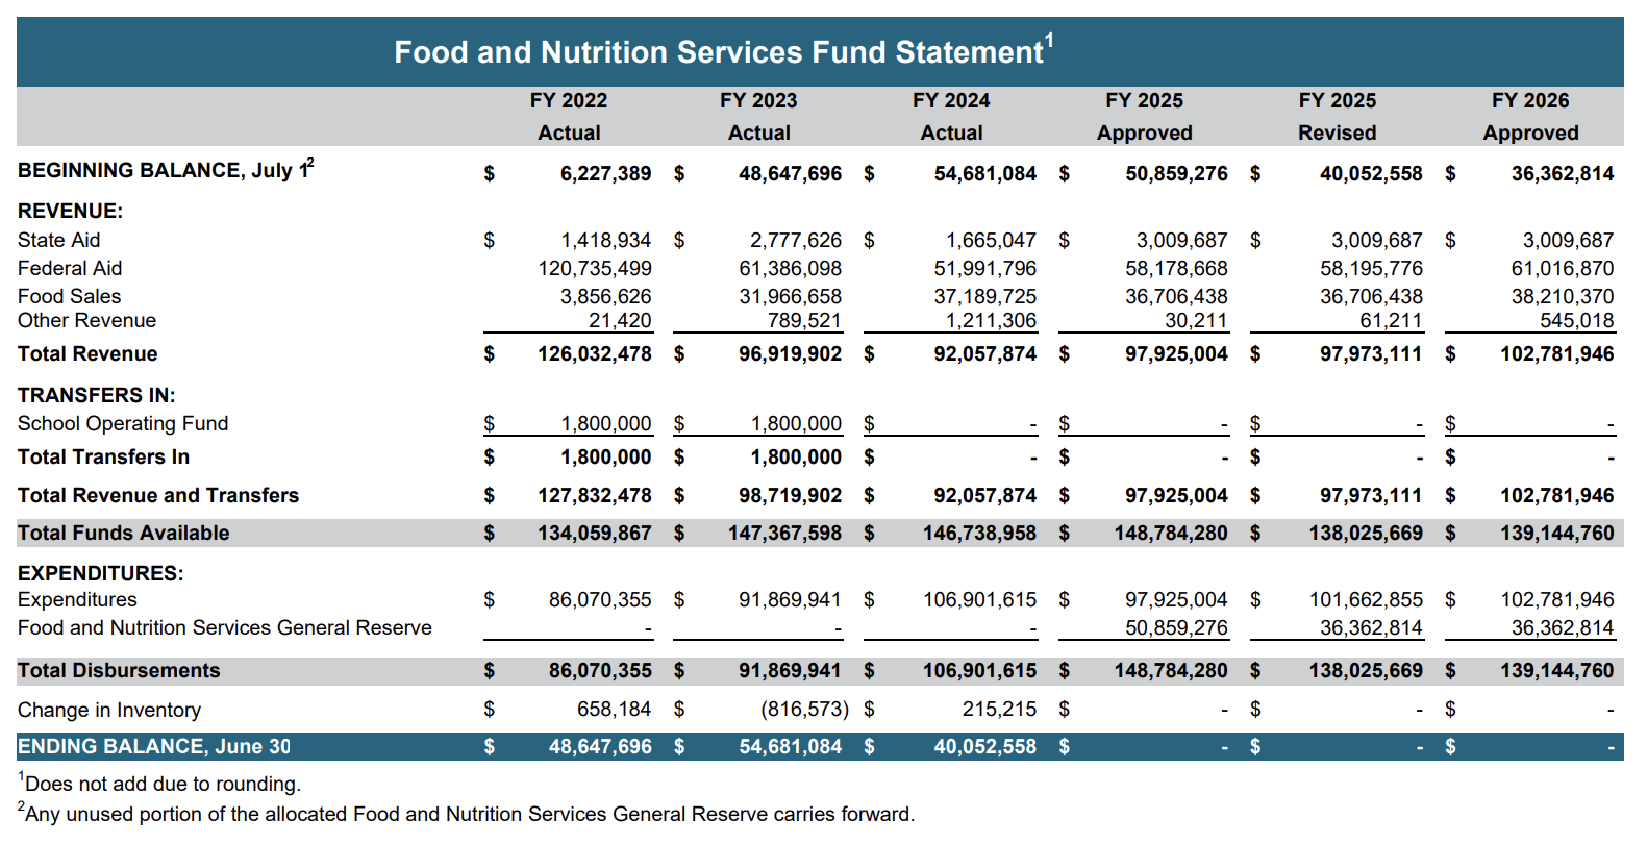
\includegraphics[scale=0.5]{fig/fcps_2026_budget.eps}
	\end{center}
	\caption{Food and Nutrition Services Fund Statement from FCPS’ 2026 Approved Budget document}
	\label{fig:fcpsbudget}
\end{figure}

When determining the budget for the optimization model, the value was used based on the 2026 approved budget total funds available value. This value was what the Food and Nutrition Services had to work with, so this provided a realistic target for the optimization model.


\subsection{Data tables}

\begin{table}[H]
    \centering
    \renewcommand{\arraystretch}{1.5}

    \textbf{\large unit\_costs.csv}
    \vspace{0.2cm}

    \begin{tabular}{|>{\columncolor{lightgray!50}\bfseries}r|l|r|}
    \hline
        \rowcolor{lightgray!50} % Darker gray for the header row
        \textbf{identifier} & \textbf{name} & \textbf{unit\_cost} \\ 
        \hline
        10064 & -Peas and Diced Carrots, Frozen (1/2 cup) & 0 \\
        \hline
        30102 & 1\% Unflavored Shelf-Stable Milk (Each) & 0.38 \\
        \hline
        20001 & 1\% White Milk (Each) & 0.36 \\
        \hline
        60128 & Alfredo \& Basil Lasagna (Each) & 1.26 \\
        \hline
    \end{tabular}

    \caption{Structure of the ``unit\_costs.csv'' file}
    \label{tab:unitcost}
\end{table}

The unit\_costs.csv file contains the unit cost of individual menu items. The identifier values allow the items to be linked back to other files, allowing joins to provide detailed analysis.

% Start Landscape Mode
\begin{landscape}
    \vspace*{\fill}
    \begin{table}[H]
        \centering
        \tiny
        \setlength{\tabcolsep}{1pt}
        \renewcommand{\arraystretch}{1.2}

        \textbf{\large data\_breakfast.csv}
        \vspace{0.2cm}

        \makebox[\textwidth][c]{
        \begin{tabular}{|l|c|c|l|r|r|r|r|r|r|r|r|r|r|r|r|r|r|r|r|}
            \hline
            \rowcolor{lightgray!50}
            % Headers with manual line breaks to save space
            \textbf{School} & 
            \textbf{Date} & 
            \textbf{ID} & 
            \textbf{Item Name} & 
            \textbf{\shortstack{Plan\\Reimb}} & 
            \textbf{\shortstack{Plan\\Non-reimb}} & 
            \textbf{\shortstack{Plan\\Total}} & 
            \textbf{Offered} & 
            \textbf{\shortstack{Served\\Reimb}} & 
            \textbf{\shortstack{Served\\Non-reimb}} & 
            \textbf{\shortstack{Served\\Total}} & 
            \textbf{\shortstack{Served\\Cost}} & 
            \textbf{\shortstack{Discarded\\Total}} & 
            \textbf{\shortstack{Discarded\\\% of Offered}} & 
            \textbf{\shortstack{Discarded\\Cost}} & 
            \textbf{\shortstack{Subtotal\\Cost}} & 
            \textbf{\shortstack{Leftover\\Total}} & 
            \textbf{\shortstack{Leftover\\\% of Offered}} & 
            \textbf{\shortstack{Leftover\\Cost}} & 
            \textbf{\shortstack{Production\\Cost Total}} \\ 
            \hline
            
            Aldrin Elementary & 2025-05-01 & 20001 & 1\% White Milk & 33 & 0 & 33 & 37 & 34 & 0 & 34 & \$12.24 & 0 & 0.00\% & \$0.00 & \$12.24 & 3 & 8.11\% & \$1.08 & \$13.32 \\ 
            \hline

            Aldrin Elementary & 2025-05-01 & 30008 & Apple Juice & 43 & 0 & 43 & 55 & 50 & 0 & 50 & \$8.50 & 0 & 0.00\% & \$0.00 & \$8.50 & 5 & 9.09\% & \$0.85 & \$9.35 \\ 
            \hline

            Aldrin Elementary & 2025-05-01 & 60089 & Assorted Cereal & 0 & 0 & 0 & 10 & 4 & 0 & 4 & \$2.36 & 0 & 0.00\% & \$0.00 & \$2.36 & 6 & 60.00\% & \$3.54 & \$5.90 \\ 
            \hline

            Aldrin Elementary & 2025-05-01 & 30004 & Blueberry Chex & 11 & 0 & 11 & 10 & 8 & 0 & 8 & \$4.72 & 0 & 0.00\% & \$0.00 & \$4.72 & 0 & 0.00\% & \$0.00 & \$4.72  \\ 
            \hline

            Aldrin Elementary & 2025-05-01 & 30068 & Chilled Peaches & 13 & 0 & 13 & 12 & 11 & 0 & 11 & \$5.61 & 0 & 0.00\% & \$0.00 & \$5.61 & 1 & 8.33\% & \$0.51 & \$6.12 \\
            \hline

            Aldrin Elementary & 2025-05-01 & 30006 & Cinnamon Chex Cereal & 12 & 0 & 12 & 10 & 8 & 0 & 8 & \$4.72 & 0 & 0.00\% & \$0.00 & \$4.72 & 2 & 20.00\% & \$1.18 & \$5.90 \\
            \hline

            Aldrin Elementary & 2025-05-01 & 30007 & Cinnamon Toast Crunch & 13 & 0 & 13 & 10 & 5 & 0 & 5 & \$2.95 & 0 & 0.00\% & \$0.00 & \$2.95 & 5 & 50.00\% & \$2.95 & \$5.90 \\
            \hline

            Aldrin Elementary & 2025-05-01 & 60125 & Egg and Cheese Biscuit & 10 & 0 & 10 & 7 & 4 & 0 & 4 & \$1.88 & 1 & 14.29\% & \$0.47 & \$2.35 & 2 & 28.57\% & \$0.94 & \$3.29 \\
            \hline

            Aldrin Elementary & 2025-05-01 & 20038 & Fat Free White Milk & 11 & 0 & 11 & 15 & 13 & 0 & 13 & \$4.29 & 0 & 0.00\% & \$0.00 & \$4.29 & 2 & 13.33\% & \$0.66 & \$4.95 \\
            \hline
            
        \end{tabular}
        }
        
        \caption{Structure of data\_breakfast.csv file (same as data\_lunch.csv)}
        \label{tab:breakfast_structure}
    \end{table}

    \vspace{1cm}
    
    \begin{table}[H]
        \centering
        \tiny % Smallest font size
        \setlength{\tabcolsep}{1.5pt} % Tight spacing between columns
        \renewcommand{\arraystretch}{1.2}

            \textbf{\large sales.csv}
        \vspace{0.2cm}
        
        % Force horizontal centering relative to the page, not margins
        \makebox[\textwidth][c]{
            \begin{tabular}{|l|c|l|c|c|l|r|r|r|r|r|r|r|r|r|r|r|r|r|}
                \hline
                \rowcolor{lightgray!50}
                % Headers using shortstack to save horizontal space
                \textbf{\shortstack{Time of Day}} & 
                \textbf{\shortstack{School\\Code}} & 
                \textbf{School Name} & 
                \textbf{Date} & 
                \textbf{Item} & 
                \textbf{Description} & 
                \textbf{Total} & 
                \textbf{Free Meals} & 
                \textbf{\shortstack{Reduced Price}} & 
                \textbf{\shortstack{Full Price}} & 
                \textbf{Adults} & 
                \textbf{\shortstack{Alac\\Student}} & 
                \textbf{\shortstack{Alac\\Adult}} & 
                \textbf{\shortstack{Earned\\Student}} & 
                \textbf{\shortstack{Earned\\Adult}} & 
                \textbf{\shortstack{Earned Alac\\Student}} & 
                \textbf{\shortstack{Earned Alac\\Adult}} & 
                \textbf{\shortstack{Adj\\Alac}} & 
                \textbf{\shortstack{Adj\\Meal}} \\ 
                \hline

                breakfast & 17 & Colvin Run Elementary & 5/1/25 & 1146 & Cereal Meal & 10 & 2 & 0 & 8 & 0 & 0 & 0 & 0 & 0 & 0 & 0 & 0 & 0 \\ 
                \hline
                
                breakfast & 17 & Colvin Run Elementary & 5/1/25 & 1170 & Mini Pancakes & 32 & 2 & 0 & 30 & 0 & 0 & 0 & 0 & 0 & 0 & 0 & 0 & 0 \\ 
                \hline
                
                breakfast & 17 & Colvin Run Elementary & 5/1/25 & 1310 & ALC Breakfast Entree & 8 & 0 & 0 & 0 & 0 & 8 & 0 & 0 & 0 & 0 & 0 & 0 & 0 \\ 
                \hline

                breakfast & 17 & Colvin Run Elementary & 5/1/25 & 1405 & Egg and Cheese Biscuit & 2 & 0 & 0 & 2 & 0 & 0 & 0 & 0 & 0 & 0 & 0 & 0 & 0 \\ 
                \hline

                breakfast & 17 & Colvin Run Elementary & 5/1/25 & 151 & Cereal/No Milk & 9 & 0 & 0 & 0 & 0 & 9 & 0 & 0 & 0 & 0 & 0 & 0 & 0 \\
                \hline

                breakfast & 17 & Colvin Run Elementary & 5/1/25 & 188 & \$1.00 Water 16.9oz & 1 & 0 & 0 & 0 & 0 & 1 & 0 & 0 & 0 & 0 & 0 & 0 & 0 \\
                \hline
                
                breakfast & 17 & Colvin Run Elementary & 5/1/25 & 700 & ALC Milk & 1 & 0 & 0 & 0 & 0 & 1 & 0 & 0 & 0 & 0 & 0 & 0 & 0 \\
                \hline

                breakfast & 17 & Colvin Run Elementary & 5/1/25 & 717 & ALC Juice 4oz \$.75 & 30 & 0 & 0 & 0 & 0 & 30 & 0 & 0 & 0 & 0 & 0 & 0 & 0 \\
                \hline
                
            \end{tabular}
        }
        
        \caption{Structure of sales.csv file}
        \label{tab:sales_structure}
    \end{table}

    \vspace*{\fill} % Centers vertically (Top to Bottom)
\end{landscape}

From \autoref{tab:breakfast_structure}, the \texttt{data\_breakfast.csv} and \texttt{data\_lunch.csv} files are the main data files that are produced by the \texttt{data\_transformer\_html} and \texttt{csv\_combiner} programs. The features in the csv file are as follows:

\begin{itemize}
    \item \textbf{school\_name}: The name of the school
    \item \textbf{date}: The specific date for which the data is recorded
    \item \textbf{identifier}: A unique ID
    \item \textbf{name}: The name of the item being tracked
    \item \textbf{planned\_reimbursable}: The number of items planned for students
    \item \textbf{planned\_non-reimbursable}: The number of items planned for others
    \item \textbf{planned\_total}: The total number of items planned (reimbursable + non-reimbursable)
    \item \textbf{offered}: The total number of items made available for selection
    \item \textbf{served\_reimbursable}: The number of items actually served to students
    \item \textbf{served\_non-reimbursable}: The number of items actually served to others
    \item \textbf{served\_total}: The total number of items served (reimbursable + non-reimbursable)
    \item \textbf{served\_cost}: The total cost of the items that were served
    \item \textbf{discarded\_total}: The number of items thrown away or not used
    \item \textbf{discarded\_percent\_of\_offered}: The percentage of offered items that were discarded
    \item \textbf{discarded\_cost}: The cost associated with the discarded items
    \item \textbf{subtotal\_cost}: The combined cost before adding production costs
    \item \textbf{left\_over\_total}: The number of unused items that were not served but not discarded
    \item \textbf{left\_over\_percent\_of\_offered}: The percentage of offered items that were left over
\end{itemize}

In \autoref{tab:sales_structure}, the \texttt{sales.csv} file is created by the \texttt{pdf\_processor} program. The features in the csv file are as follows:

\begin{itemize}
    \item \textbf{time\_of\_day}: The meal period or service time (e.g., breakfast, lunch)
    \item \textbf{school\_code}: A unique code identifying the school
    \item \textbf{school\_name}: The name of the school associated with the record
    \item \textbf{date}: The date on which the item data was recorded
    \item \textbf{item}: The item name being tracked
    \item \textbf{description}: Additional details about the item
    \item \textbf{total}: The total number of items served
    \item \textbf{free\_meals}: The number of meals served to students qualifying for free meals
    \item \textbf{reduced\_price\_meals}: The number of meals served to students qualifying for reduced-price meals
    \item \textbf{full\_price\_meals}: The number of meals served to students paying full price
    \item \textbf{adults}: The number of meals served to adults (staff or visitors)
    \item \textbf{alac\_student}: The number of à la carte items sold to students
    \item \textbf{alac\_adult}: The number of à la carte items sold to adults
    \item \textbf{earned\_student}: Revenue earned from student meals
    \item \textbf{earned\_adult}: Revenue earned from adult meals
    \item \textbf{earned\_alac\_student}: Revenue earned from student à la carte sales
    \item \textbf{earned\_alac\_adult}: Revenue earned from adult à la carte sales
    \item \textbf{adj\_alac}: Adjustments made to à la carte counts
    \item \textbf{adj\_meal}: Adjustments made to meal counts
\end{itemize}

\begin{table}[H]
    \centering
    \renewcommand{\arraystretch}{1.5}

    \textbf{\large 2022-2025 Fairfax County School Student Count}
    \vspace{0.2cm}

    \begin{tabular}{|>{\columncolor{lightgray!50}\bfseries}l|r|r|r|}
    \hline
        \rowcolor{lightgray!50} % Darker gray for the header row
        School\_Name & \textbf{2022-2023} & \textbf{2023-2024} & \textbf{2024-2025} \\ 
        \hline
        Aldrin Elementary & 641 & 655 & 652 \\ 
        \hline
        Annandale High & 2937 & 3027 & 2945 \\ 
        \hline
        Annandale Terrace Elementary & 1233 & 1309 & 1282 \\ 
        \hline
        Armstrong Elementary & 565 & 594 & 556 \\ 
        \hline
        Baileys Lower Elementary & 1373 & 1464 & 1408 \\ 
        \hline
        Baileys Upper Elementary & 1135 & 1099 & 1056 \\ 
        \hline
    \end{tabular}

    \caption{Structure of ``2022-2025 Fairfax County School Student Count.csv'' file}
    \label{tab:student_count}
\end{table}

The 2022-2025 Fairfax County School Student Count.csv file contains data of student population sizes for each individual school according to the year. We researched this data from the School Profiles page provided by Fairfax County Public Schools \cite{fcps_profiles}. The numbers calculated are the sum of the enrollment numbers of all the categories that are listed on the table.

\subsection{Graphs}

\begin{figure}[H]
	\begin{center}
		
\includegraphics[scale=0.3]{fig/savings_analysis_color.eps}
	\end{center}
	\caption{Bubble graph of the savings analysis between actual and optimized production costs}
	\label{fig:overallsavings}
\end{figure}

\autoref{fig:overallsavings} compares the results of the savings between actual and optimized production costs for each individual school in the Fairfax County Public School system. The dashed line going across represents the zero mark where there would be no money being saved. Data points below the line represent the schools that are saving with the optimization model, where the bigger the bubble, the bigger the savings. Data points above the line represent schools that are losing money with the optimization model, where the bigger the bubble, the bigger the loss is. The figure shows that the majority of the schools are showing positive results with the optimization model, whereas 60 schools are showing negative results.

It is important to consider the schools below the line as this shows that the model is optimizing that results in savings. \autoref{tab:schoolsavings} shows the schools that benefit from our optimization model (Baseline Budget):

\setlength\LTleft{0pt}
\setlength\LTright{0pt}

\renewcommand{\arraystretch}{1.4}
\begin{longtable}{|>{\raggedright\arraybackslash}p{0.3\textwidth}|>{\raggedright\arraybackslash}p{0.3\textwidth}|>{\raggedright\arraybackslash}p{0.3\textwidth}|}
    \hline
    \rowcolor{lightgray!50}
    \multicolumn{3}{|c|}{\textbf{Baseline Budget: Schools with Savings from Optimizer}} \\
    \hline
    \endfirsthead
    
    \hline
    \rowcolor{lightgray!50}
    \multicolumn{3}{|c|}{\textit{...continued from previous page}} \\
    \hline
    \endhead
    
    \hline
    \multicolumn{3}{|r|}{\textit{Continued on next page...}} \\
    \endfoot
    
    \hline
    \endlastfoot

    Franklin Sherman Elementary & Vienna Elementary & Little Run Elementary \\
    \hline
    Chesterbrook Elementary & Armstrong Elementary & Olde Creek Elementary \\
    \hline
    Lees Corner Elementary & Flint Hill Elementary & Kings Glen Elementary \\
    \hline
    Rolling Valley Elementary & Great Falls Elementary & Fort Hunt Elementary \\
    \hline
    Columbia Elementary & Waynewood Elementary & Haycock Elementary \\
    \hline
    Clermont Elementary & Cunningham Park Elem. & Forestville Elementary \\ 
    \hline
    West Springfield Elem. & Wakefield Forest Elem. & Poplar Tree Elementary \\ 
    \hline
    Fox Mill Elementary & Franconia Elementary & Ravensworth Elementary \\ 
    \hline
    Colvin Run Elementary & Mcnair Upper Elem. & Springfield Estates Elem. \\ 
    \hline
    Hayfield Elementary & Waples Mill Elementary & Newington Forest Elem. \\ 
    \hline
    Garfield Elementary & Oak Hill Elementary & Stratford Landing Elem. \\ 
    \hline
    Floris Elementary & Churchill Road Elem. & Lemon Road Elementary \\ 
    \hline
    Fairhill Elementary & Terra Centre Elementary & Oak View Elementary \\
    \hline
    Marshall Road Elementary & Greenbriar West Elementary & Stenwood Elementary \\
    \hline
    Union Mill Elementary & Gunston Elementary & Bucknell Elementary \\
    \hline
    Freedom Hill Elementary & North Springfield Elementary & Bush Hill Elementary \\
    \hline
    Cub Run Elementary & Navy Elementary & Terraset Elementary \\
    \hline
    Westgate Elementary & Shrevewood Elementary & Eagle View Elementary \\
    \hline
    Saratoga Elementary & Halley Elementary & Kent Gardens Elementary \\
    \hline
    Woodlawn Elementary & Jefferson High & Orange Hunt Elementary \\
    \hline
    Mcnair Elementary & Mantua Elementary & Deer Park Elementary \\
    \hline
    Lane Elementary & Lake Anne Elementary & Laurel Ridge Elementary \\
    \hline
    Forest Edge Elementary & Dranesville Elementary & Fort Belvoir Upper Elementary \\
    \hline
    Virginia Run Elementary & Laurel Hill Elementary & Camelot Elementary \\
    \hline
    Lorton Station Elementary & Woodburn Elementary & Forestdale Elementary \\
    \hline
    Bull Run Elementary & Graham Road Elementary & Beech Tree Elementary \\
    \hline
    Centreville Elementary & Sangster Elementary & Daniels Run Elementary \\
    \hline
    Timber Lane Elementary & Woodley Hills Elementary & Madison High \\
    \hline
    Greenbriar East Elementary & Belvedere Elementary & Mosaic Elementary \\
    \hline
    Mt. Vernon Woods Elementary & Providence Elementary & Franklin Middle \\
    \hline
    Twain Middle & Sleepy Hollow Elementary & South County Middle \\
    \hline
    Kings Park Elementary & Riverside Elementary & Hollin Meadows Elementary \\
    \hline
    Sandburg Middle & Clearview Elementary & Annandale Terrace Elementary \\
    \hline
    West Lawn Elementary & Cameron Elementary & Fort Belvoir Primary Elementary \\
    \hline
    Centre Ridge Elementary & Langley High & Brookfield Elementary \\
    \hline
    Crestwood Elementary & Lynbrook Elementary & Mason Crest Elementary \\
    \hline
    Pine Spring Elementary & London Towne Elementary & Luther Jackson Middle \\
    \hline
    Herndon Elementary & Weyanoke Elementary & Glen Forest Elementary \\
    \hline
    Baileys Upper Elementary & Groveton Elementary & Dogwood Elementary \\
    \hline
    Poe Middle & Baileys Lower Elementary & Hybla Valley Elementary \\
    \hline
    Hutchison Elementary & Braddock Elementary & Holmes Middle \\
    \hline
    Glasgow Middle & Westfield High & Oakton High \\
    \hline
    Chantilly High & Parklawn Elementary & Coates Elementary \\
    \hline
    Falls Church High & & \\
    \hline
    \caption{Schools that are saving from our model under the baseline budget}
    \label{tab:schoolsavings}
\end{longtable}


\begin{figure}[H]
	\begin{center}
		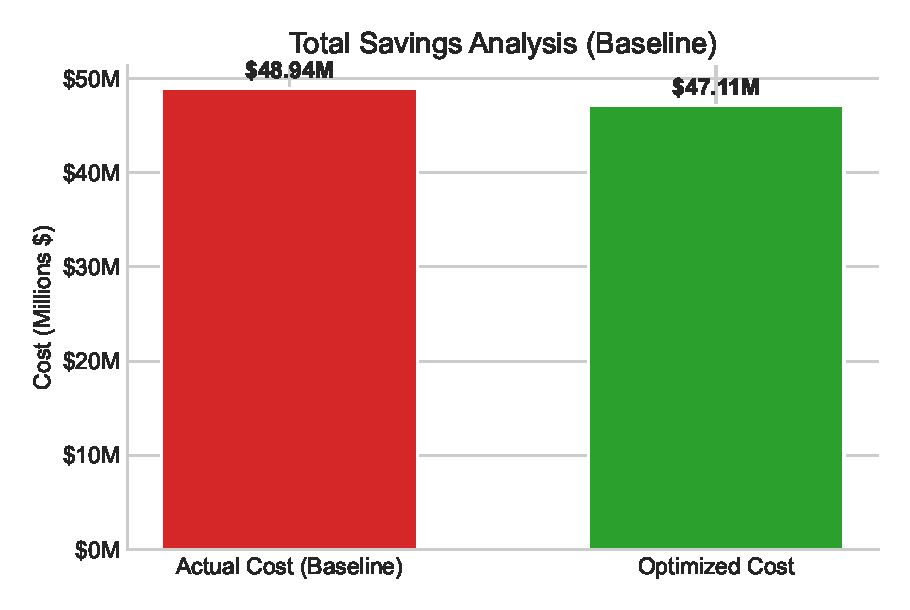
\includegraphics[scale=0.7]{fig/total_savings_bar_color.eps}
	\end{center}
	\caption{Bar graph of overall savings: actual vs. optimized annual food costs}
	\label{fig:totalsavingsbar}
\end{figure}

Considering the results from the optimization of all schools, despite the model losing money for some schools, the model has managed to save \$1.83 million, according to \autoref{fig:totalsavingsbar}. However, overall savings can increase if FCPS continues to optimize better than our model for the other schools so that they would be saving more than what we have concluded. 

\begin{figure}[H]
	\begin{center}
		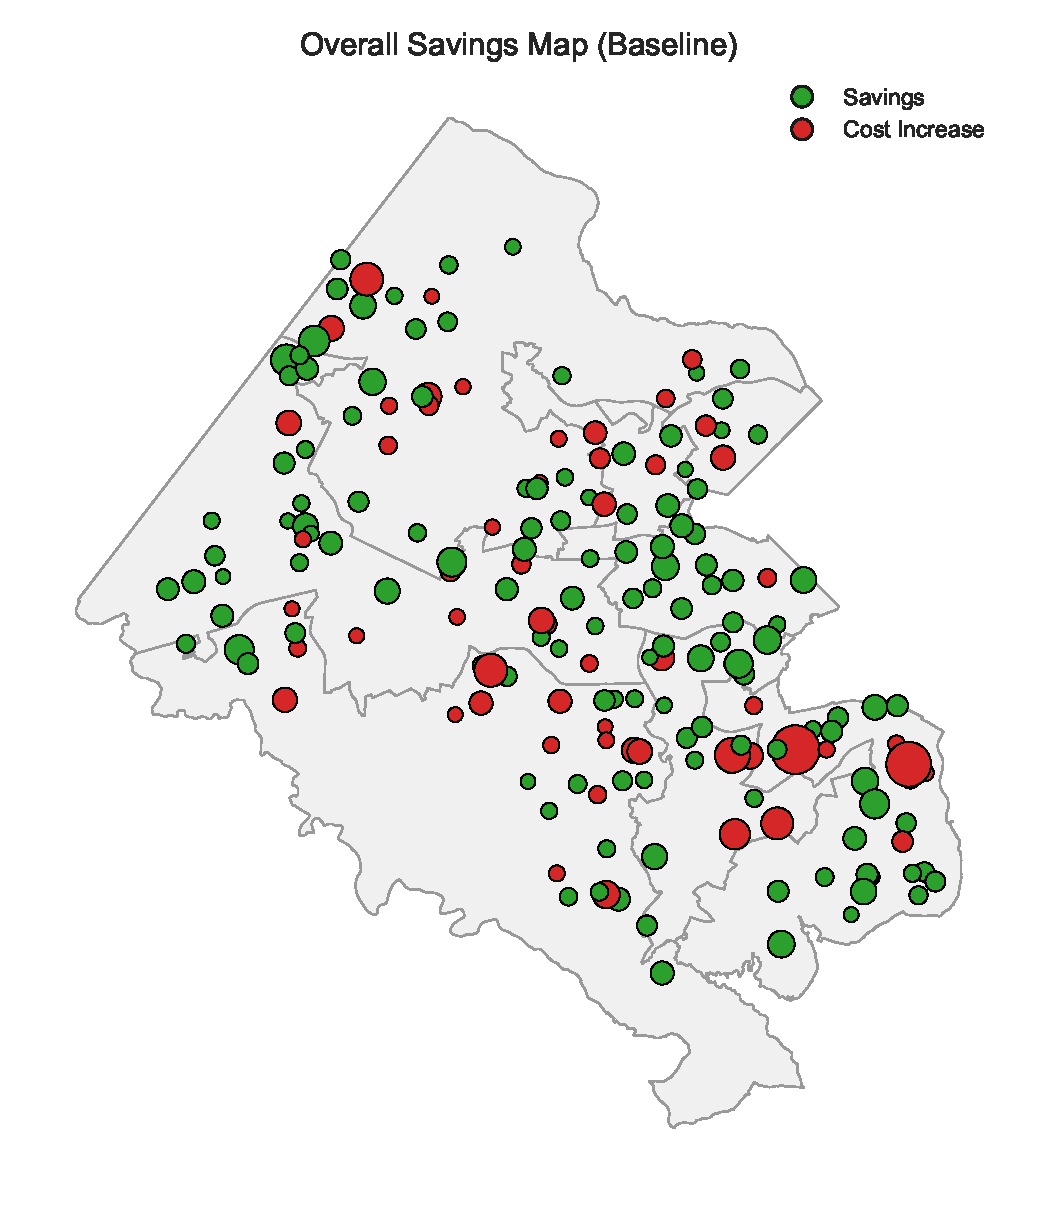
\includegraphics[scale=0.5]{fig/overall_savings_map_static.eps}
	\end{center}
	\caption{Geographical map of Fairfax County with bubbles representing the schools}
	\label{fig:geooverallsavings}
\end{figure}

\autoref{fig:geooverallsavings} provides another version of the bubble graph where green bubbles represent schools saving money from the optimization model and red representing those that are losing money from the optimization model. Through the use of a geographical map, we can observe which regions of the FCPS system contain the schools producing losses to see any trends.

\begin{figure}[H]
	\begin{center}
		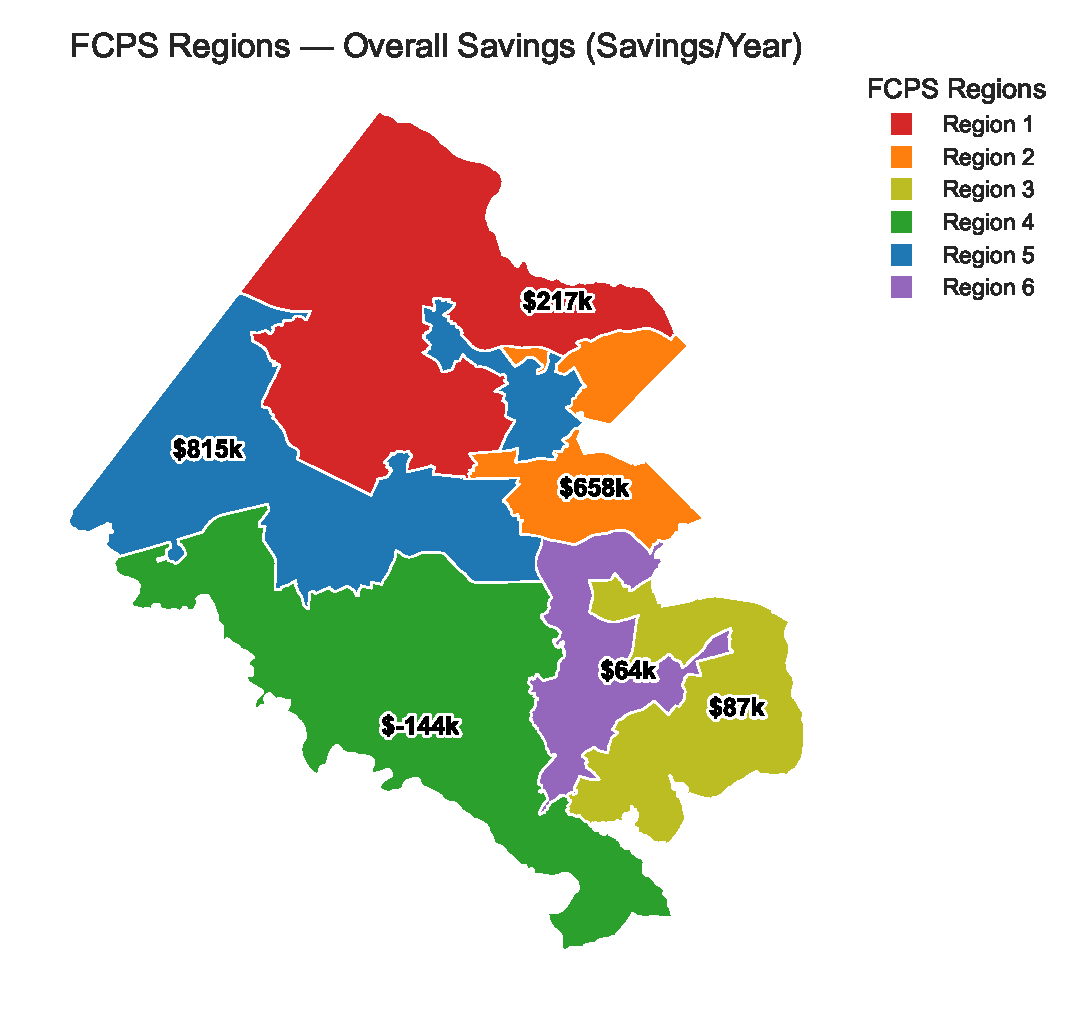
\includegraphics[scale=0.5]{fig/choropleth_overall_savings_baseline.eps}
	\end{center}
	\caption{Choropleth map of Fairfax County highlighting savings amounts from optimization}
	\label{fig:choroplethbase}
\end{figure}

\autoref{fig:choroplethbase} shows the regions of the FCPS system. We can conclude that overall regions 4 and 6 located south of the county where most of the schools are not producing high savings with the optimizer.

With the prior graphs, they showed the results from the baseline budget amount. The baseline is the normal amount of money that was allocated to schools based on the overall budget. We have also looked at a lower allocated budget and an upper allocated budget.

\begin{figure}[H] 
    \centering

    \begin{minipage}{0.49\textwidth}
        \centering
        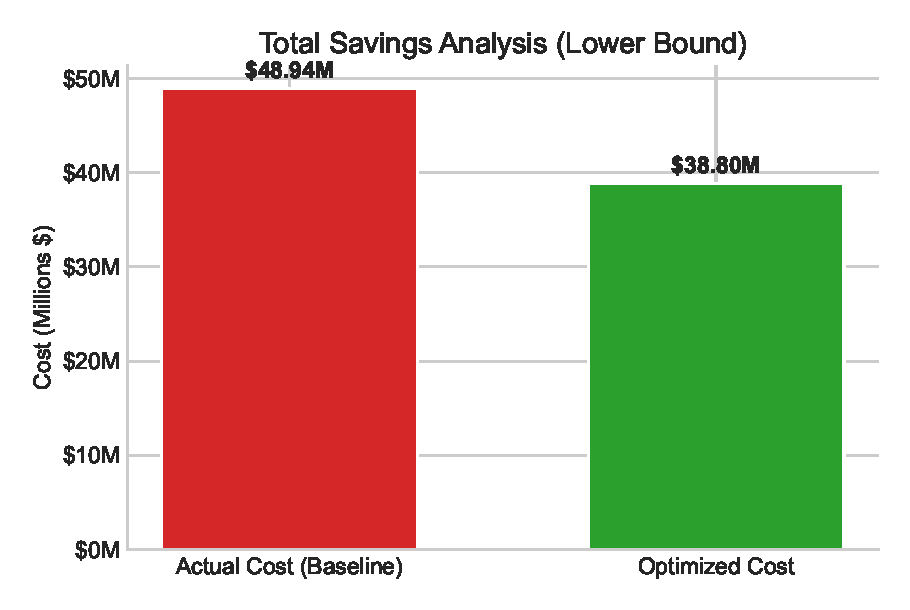
\includegraphics[width=\linewidth]{fig/total_savings_bar_color_lower_bound.eps}
    \end{minipage}
    \hfill
    \begin{minipage}{0.49\textwidth}
        \centering
        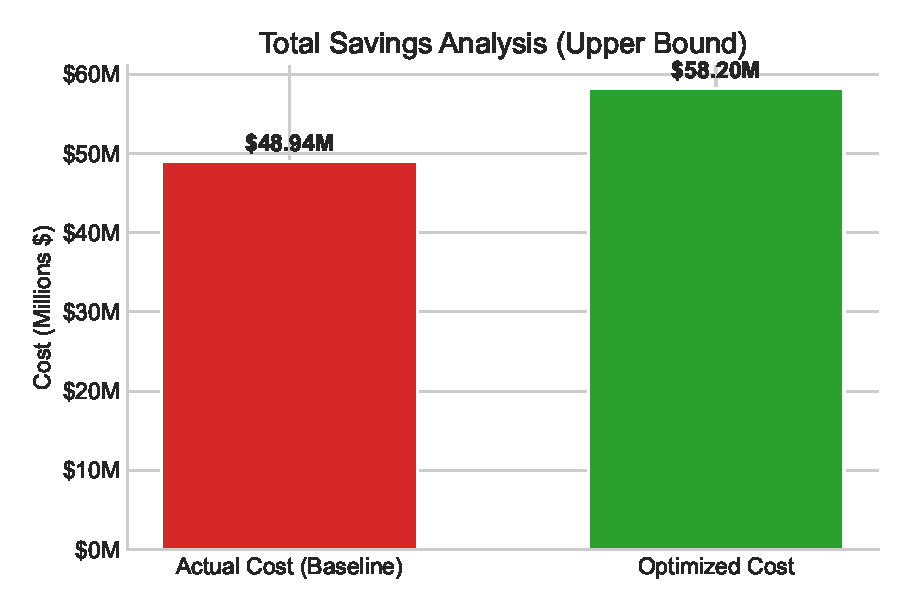
\includegraphics[width=\linewidth]{fig/total_savings_bar_color_upper_bound.eps}
    \end{minipage}

    \caption{Lower (left) \& Upper (right) Bound Budget Scenario: Actual vs Optimized Costs}
    \label{fig:lower_upper_budget}
\end{figure}

\begin{figure}[H] 
    \centering

    \begin{minipage}{0.49\textwidth}
        \centering
        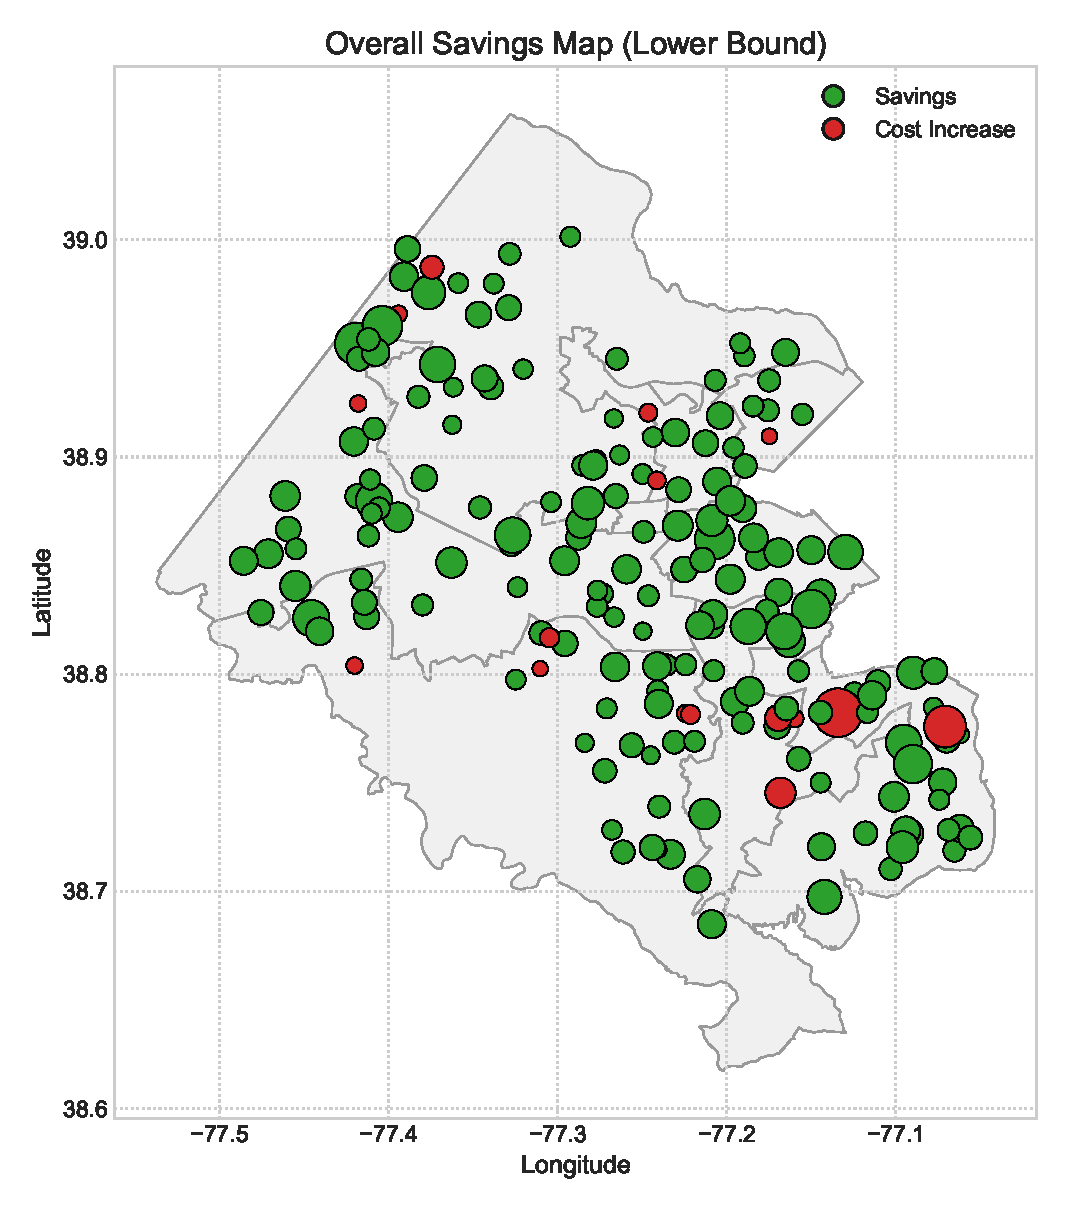
\includegraphics[width=\linewidth]{fig/choropleth_overall_savings_lower_bound.eps}
    \end{minipage}
    \hfill
    \begin{minipage}{0.49\textwidth}
        \centering
        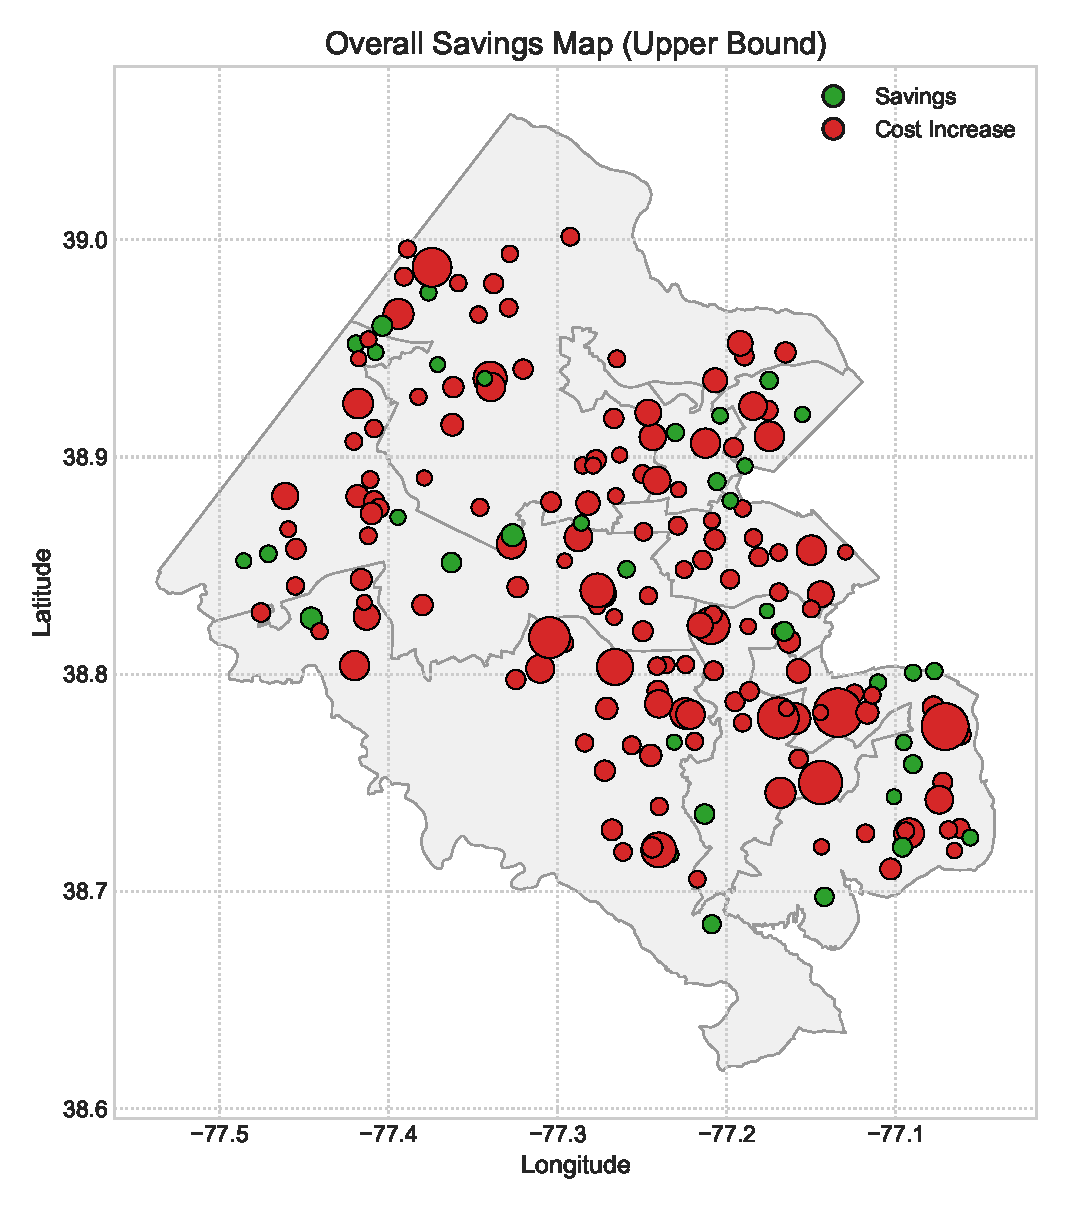
\includegraphics[width=\linewidth]{fig/choropleth_overall_savings_upper_bound.eps}
    \end{minipage}

    \caption{Lower (left) \& Upper (right) Bound Budget Scenario: Geographical Map of Fairfax County of Optimization Savings}
    \label{fig:choropleth_lower_upper}
\end{figure}

Seeing both bounds of the budget, we see both extremes of savings and loss making a prominent appearance in either graph. It is understandable that when the budget is set too low, then there will be massive savings when compared to the historical actual cost, and vice versa. However, both come in with risks. For the lower bound budget scenario, even though it is resulting in massive savings, it is risking not having enough food for their students. This would be a major problem as no child should go hungry while in school. For the upper bound budget scenario, it allows schools to produce more food, avoiding the possibility of leaving students hungry. However, that would result in a lot of food not being consumed by students, therefore, producing a lot of waste. It is helpful to know both of these extremes as going to the best of both ends points us to the baseline amount

% ------------------------------------------------------------------------------------------------------------------------

\section{Discussion}

\subsection{Comparison to Behavioral and Post-Consumer Approaches}

Our approach represents a shift from the descriptive and behavioral methodologies prominent in school food waste literature. Studies by Martins et al. and Rada et al. successfully identified factors influencing waste—such as cafeteria crowding and student age—but relied heavily on manual auditing and surveys \cite{factors, rada}. While valuable for diagnosing the "why" behind waste, these methods are resource-intensive and do not provide an automated mechanism for daily production planning. Similarly, while Elnakib et al. demonstrated that staff training and "Smarter Lunchrooms" nudges can reduce waste by ~7\%, these interventions depend on human consistency and continuous enforcement \cite{elnakib}. By contrast, MILP model offers a systematic, prescriptive solution. It automates the decision-making process, ensuring that production matches historical trends regardless of staff turnover or daily behavioral fluctuations.

Furthermore, our model targets pre-consumer waste reduction (source reduction), which distinguishes it from the MILP applications conducted by Kabadurmus et al. and Korcyl, Ksi{\k{a}}{\.z}ek, and Gdowska \cite{kabadurmus, korcyl}. Those studies utilized optimization to manage waste after it was generated, focusing on reverse logistics to food banks or recycling centers. While effective for circular economy goals, our approach arguably targets a higher priority in the waste hierarchy: preventing surplus production entirely.

\subsection{Trade-offs and Methodological Limitations}

However, there are areas where alternative approaches outperform our deterministic model. As noted by G{\"u}nder et al. exact MILP methods can struggle with the non-linear biological complexities found in agricultural harvest scheduling, where Evolutionary Algorithms proved superior \cite{gunder}. While our school cafeteria setting is currently modeled with linear constraints, future attempts to integrate "farm-to-school" supply chains—with their inherent biological variability—might require shifting from our exact ILP model to the stochastic meta-heuristics suggested by G{\"u}nder et al. \cite{gunder}.

Additionally, our focus on supply-side optimization ignores the demand-side behavioral levers identified by Martins et al. and Rada et al. \cite{factors, rada}. Our model can optimize how much pizza to make, but it cannot influence how much of that pizza a student actually eats. A truly holistic system would likely need to couple our production optimization with the educational interventions proposed by Rada et al. to tackle both production surplus and plate waste simultaneously \cite{rada}.

\subsection{Data Constraints and Demand Uncertainty}

A significant challenge in this study was the reliance on production data from a single month (May 2025). As May is characterized by end-of-year testing and senior events, extrapolating these findings assumes an annual consistency that likely does not exist. Seasonal variations in attendance and food preferences could substantially alter optimal production quantities in other months. Therefore, the reported annual savings of \$1.83 million should be interpreted as a feasibility estimate based on current patterns rather than a validated projection.

Furthermore, our use of historical sales as a proxy for demand introduces the risk of "censored demand." If popular items historically stocked out, sales data would underestimate true student interest. Unlike stochastic inventory models that might estimate this lost demand, our deterministic approach risks recommending further production cuts where supply increases are actually needed. Future implementations must incorporate stockout tracking to distinguish between low demand and supply constraints.

\subsection{Financial Assumptions}

Finally, due to the structure of available budget documentation, we assumed the 'Expenditures' category primarily funded food production and was allocated proportionally to the student population. In reality, this category likely conflates variable food costs with fixed overhead (personnel, equipment). This limitation implies our cost-saving estimates may be sensitive to fixed-cost structures. Future work should seek access to line-item general ledger data, allowing the model to optimize variable food procurement independently of fixed operational expenses.

% ------------------------------------------------------------------------------------------------------------------------

\section{Conclusion}

This study utilized Mixed Integer Linear Programming to address food waste and economic inefficiency in Fairfax County Public Schools. The model projects a total annual cost reduction of \textbf{\$1.83 million} (lowering spending from \$48.94 million to \$47.11 million) while maintaining nutritional standards.

\textbf{Key Results and Observations}
\begin{itemize}
    \item \textbf{Optimal Size for Savings}: Schools with 500-1,500 students demonstrated the greatest potential for savings.
    \item \textbf{Correction of Deficits}: Larger schools showed a projected cost increase. This identifies historical under-production and ensures resources now fully meet student demand.
    \item \textbf{Feasibility}: These results demonstrate the potential magnitude of optimization, though they are subject to single month data limitations and behavioral assumptions.
\end{itemize}

\textbf{Recommendations and Future Work}: To validate these findings, we recommend a \textbf{phased implementation} in 5-10 pilot schools to refine model parameters before system-wide adoption. Future research should extend this work by:
\begin{itemize}
    \item \textbf{Incorporating Environmental Metrics}: Using MILP-based clustering to track carbon footprints and water usage \cite{oliva}.
    \item \textbf{Addressing Uncertainty}: Adopting fuzzy inventory modeling to account for demand vagueness \cite{kalaiarasi}.
    \item \textbf{Integrating Regression}: Moving the regression analysis from a descriptive role to a prescriptive one by embedding coefficients directly into the objective function.
\end{itemize}

\bibliographystyle{IEEEtran}
\bibliography{references}

\end{document} 